\documentclass[12pt,letterpaper]{article}
\usepackage{graphicx,textcomp}
\usepackage{natbib}
\usepackage{setspace}
\usepackage{fullpage}
\usepackage{color}
\usepackage[reqno]{amsmath}
\usepackage{amsthm}
\usepackage{fancyvrb}
\usepackage{amssymb,enumerate}
\usepackage[all]{xy}
\usepackage{endnotes}
\usepackage{lscape}
\newtheorem{com}{Comment}
\usepackage{float}
\usepackage{hyperref}
\newtheorem{lem} {Lemma}
\newtheorem{prop}{Proposition}
\newtheorem{thm}{Theorem}
\newtheorem{defn}{Definition}
\newtheorem{cor}{Corollary}
\newtheorem{obs}{Observation}
\usepackage[compact]{titlesec}
\usepackage{dcolumn}
\usepackage{tikz}
\usetikzlibrary{arrows}
\usepackage{multirow}
\usepackage{xcolor}
\newcolumntype{.}{D{.}{.}{-1}}
\newcolumntype{d}[1]{D{.}{.}{#1}}
\definecolor{light-gray}{gray}{0.65}
\usepackage{url}
\usepackage{listings}
\usepackage{color}

\definecolor{codegreen}{rgb}{0,0.6,0}
\definecolor{codegray}{rgb}{0.5,0.5,0.5}
\definecolor{codepurple}{rgb}{0.58,0,0.82}
\definecolor{backcolour}{rgb}{0.95,0.95,0.92}

\lstdefinestyle{mystyle}{
	backgroundcolor=\color{backcolour},   
	commentstyle=\color{codegreen},
	keywordstyle=\color{magenta},
	numberstyle=\tiny\color{codegray},
	stringstyle=\color{codepurple},
	basicstyle=\footnotesize,
	breakatwhitespace=false,         
	breaklines=true,                 
	captionpos=b,                    
	keepspaces=true,                 
	numbers=left,                    
	numbersep=5pt,                  
	showspaces=false,                
	showstringspaces=false,
	showtabs=false,                  
	tabsize=2
}
\lstset{style=mystyle}
\newcommand{\Sref}[1]{Section~\ref{#1}}
\newtheorem{hyp}{Hypothesis}

\title{Problem Set 3}
\date{Due: November 20, 2021}
\author{Linette Lim}


\begin{document}
	\maketitle
	\section*{Instructions}
	\begin{itemize}
		\item Please show your work! You may lose points by simply writing in the answer. If the problem requires you to execute commands in \texttt{R}, please include the code you used to get your answers. Please also include the \texttt{.R} file that contains your code. If you are not sure if work needs to be shown for a particular problem, please ask.
	\item Your homework should be submitted electronically on GitHub.
	\item This problem set is due before 23:59 on Sunday November 20, 2022. No late assignments will be accepted.
	\item Total available points for this homework is 80.
	\end{itemize}

		\vspace{.25cm}
	
\noindent In this problem set, you will run several regressions and create an add variable plot (see the lecture slides) in \texttt{R} using the \texttt{incumbents\_subset.csv} dataset. Include all of your code.

	\vspace{.5cm}
\section*{Question 1}
\vspace{.25cm}
\noindent We are interested in knowing how the difference in campaign spending between incumbent and challenger affects the incumbent's vote share. 
	\begin{enumerate}
		\item Run a regression where the outcome variable is \texttt{voteshare} and the explanatory variable is \texttt{difflog}.	\vspace{5cm}
\noindent First, we make sure the global environment is clear and tidyverse is loaded. Then, we enter the data.
\vspace{.5cm}
\lstinputlisting[language=R, firstline=6, lastline=6]{PS3_answers_LinetteLim.R}  
\vspace{.5cm}   
\noindent Then, we use the lm() function to fit a regression model where the outcome variable is voteshare and the explanatory variable is difflog.
\vspace{.5cm}
\lstinputlisting[language=R, firstline=10, lastline=12]{PS3_answers_LinetteLim.R}  
\vspace{.5cm}    
\noindent We get:
\begin{verbatim}
> summary(diffvote.lm)

Call:
lm(formula = voteshare ~ difflog, data = data)

Residuals:
     Min       1Q   Median       3Q      Max 
-0.26832 -0.05345 -0.00377  0.04780  0.32749 

Coefficients:
            Estimate Std. Error t value Pr(>|t|)    
(Intercept) 0.579031   0.002251  257.19   <2e-16 ***
difflog     0.041666   0.000968   43.04   <2e-16 ***
---
Signif. codes:  0 ‘***’ 0.001 ‘**’ 0.01 ‘*’ 0.05 ‘.’ 0.1 ‘ ’ 1

Residual standard error: 0.07867 on 3191 degrees of freedom
Multiple R-squared:  0.3673,	Adjusted R-squared:  0.3671 
F-statistic:  1853 on 1 and 3191 DF,  p-value: < 2.2e-16
\end{verbatim}
		\item Make a scatterplot of the two variables and add the regression line. 	\vspace{7cm}
\noindent We use the plot() function to make a scatterplot and abline () to add the regression line.
\vspace{.5cm}
\lstinputlisting[language=R, firstline=15, lastline=19]{PS3_answers_LinetteLim.R}  
\vspace{.5cm}   
\noindent We get:
\begin{figure}[hbtp!]\centering
	\caption{\footnotesize Impact of Difference in Campaign Spend on Incumbent Party Voteshare.}
	\label{fig:plot_1}
	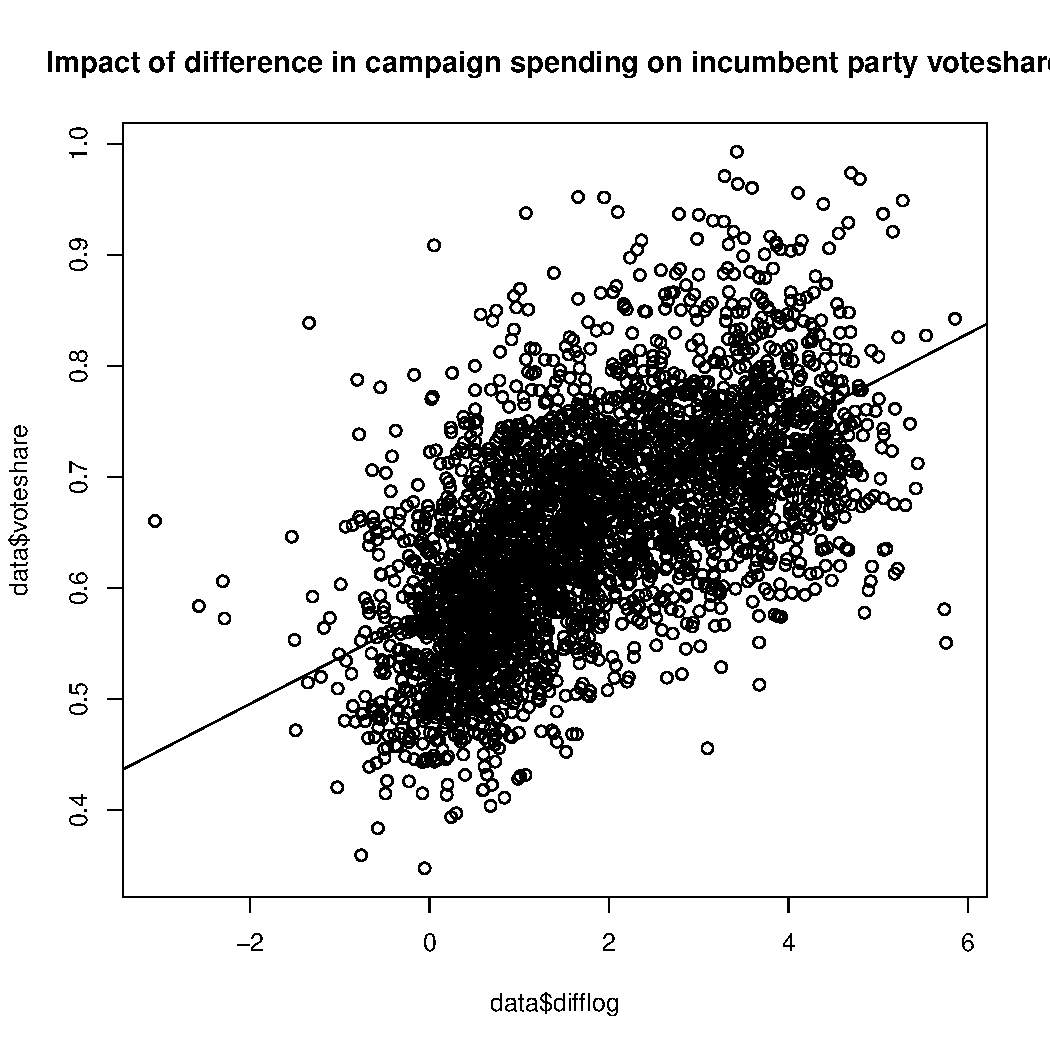
\includegraphics[width=.75\textwidth]{plot1_difflog_voteshare.pdf}
\end{figure}
		\item Save the residuals of the model in a separate object.	\vspace{7cm}
\noindent We use the resid() function to calculate the residuals and then save as separate object.
\vspace{.5cm}
\lstinputlisting[language=R, firstline=22, lastline=22]{PS3_answers_LinetteLim.R}  
\vspace{.5cm}   
\noindent Let us plot the residuals using the predict() and segments() functions to check that the assumptions of the model have been satisfied.
\vspace{.5cm}
\lstinputlisting[language=R, firstline=24, lastline=25]{PS3_answers_LinetteLim.R}  
\vspace{.5cm}   
\noindent We get:
\begin{figure}[hbtp!]\centering
	\caption{\footnotesize Residuals and regression line of Plot 1.}
	\label{fig:plot_2}
	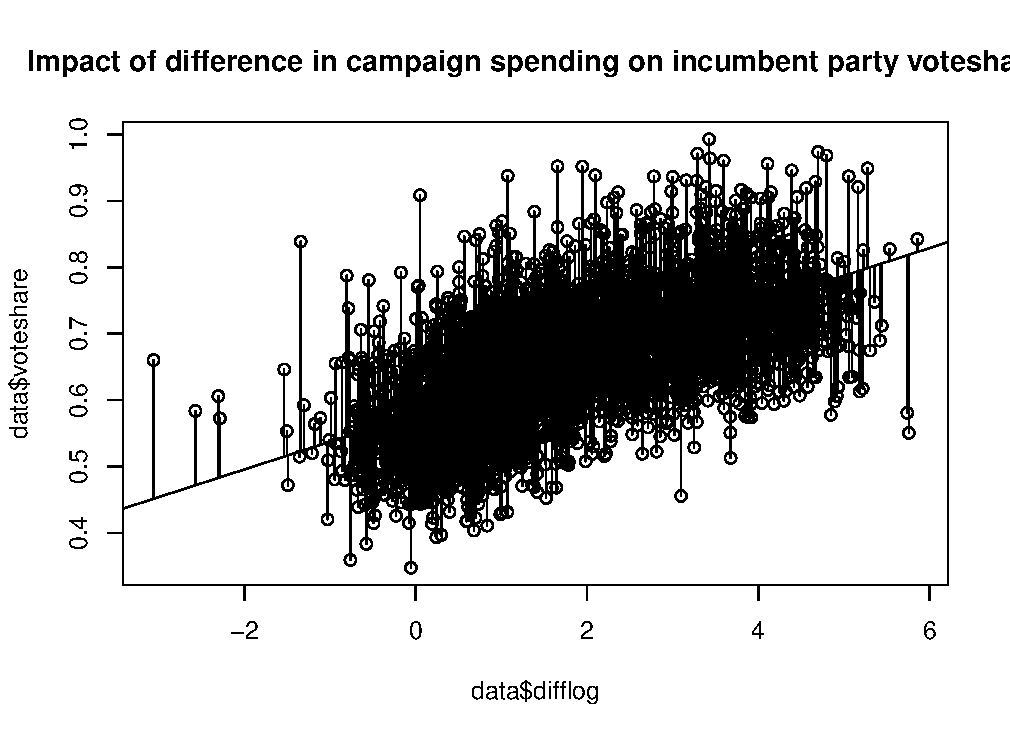
\includegraphics[width=.75\textwidth]{plot2_residuals and regression line.pdf}
\end{figure}
\noindent We want to check that the residuals are zero in expectation.
\vspace{.5cm}
\lstinputlisting[language=R, firstline=27, lastline=33]{PS3_answers_LinetteLim.R}  
\vspace{.5cm}  
\noindent We get:
\begin{figure}[hbtp!]\centering
	\caption{\footnotesize Density of residuals.}
	\label{fig:plot_3}
	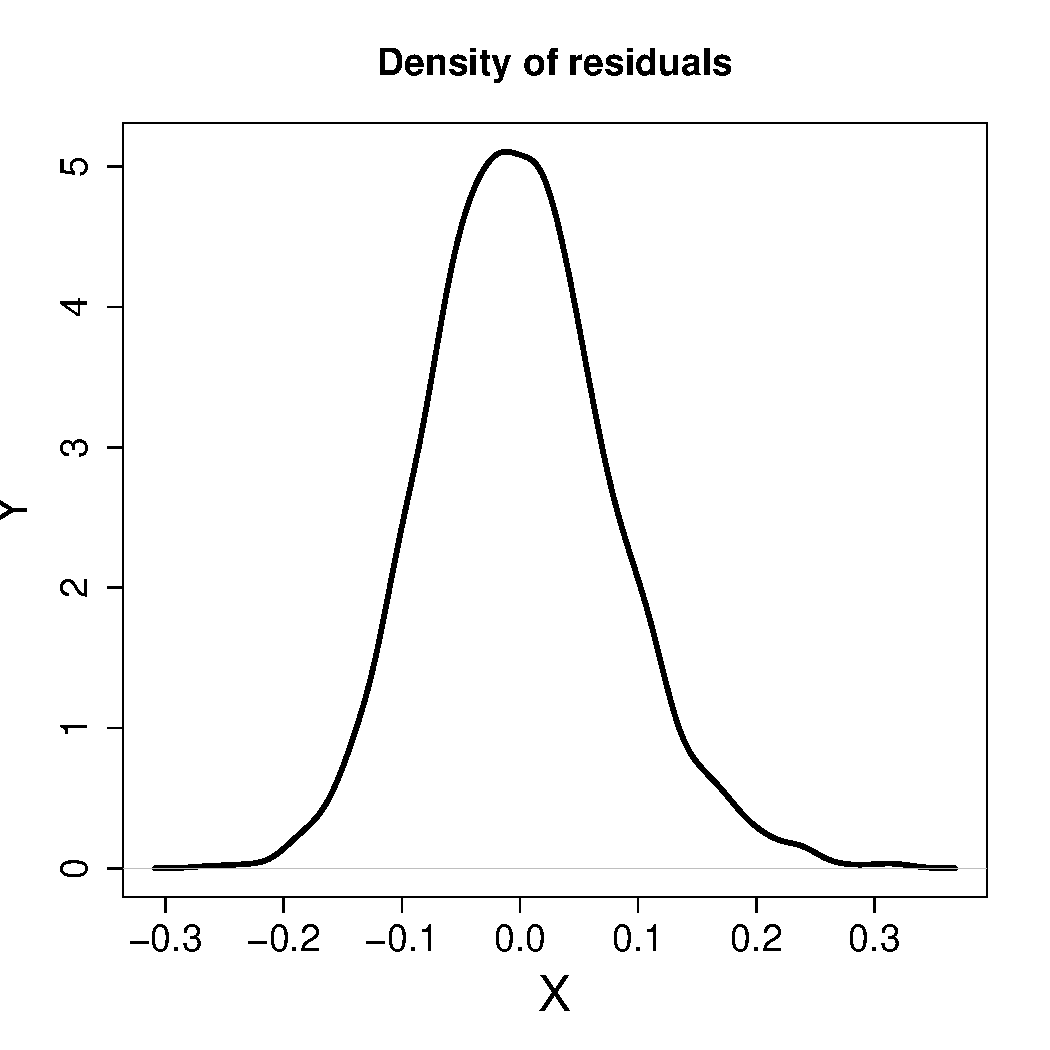
\includegraphics[width=.75\textwidth]{plot3_density of residuals.pdf}
\end{figure}
\noindent We would also expect the residuals to be randomly scattered without showing any  systematic patterns when plotted against the predictor variable:
\vspace{.5cm}
\lstinputlisting[language=R, firstline=36, lastline=39]{PS3_answers_LinetteLim.R}  
\vspace{.5cm}  
\noindent We get:
\begin{figure}[hbtp!]\centering
	\caption{\footnotesize Residual against predictor plot.}
	\label{fig:plot_4}
	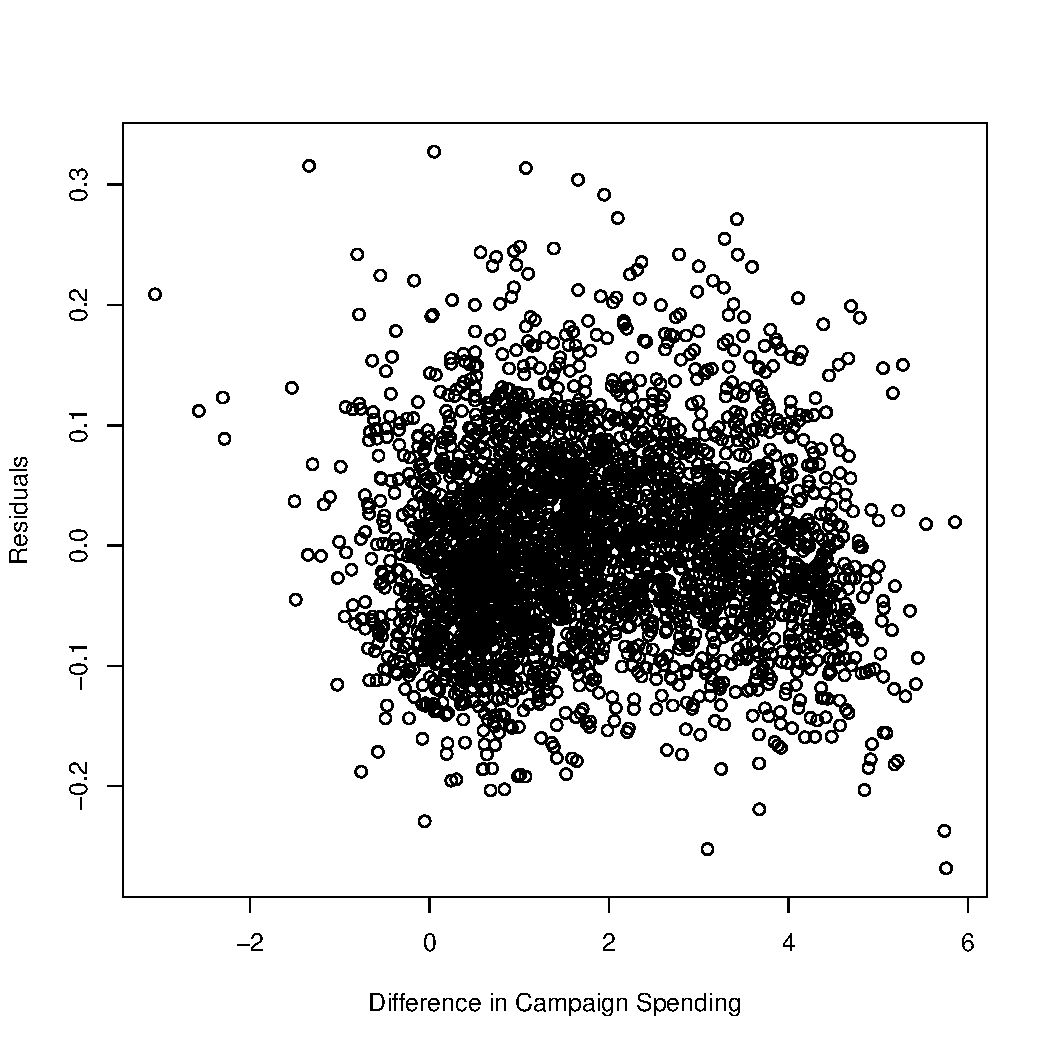
\includegraphics[width=.75\textwidth]{plot4_residual against predictor.pdf}
\end{figure}
		\item Write the prediction equation.
\noindent Using Y = b0 + b1X1 and extracting the coefficients from diffvote.lm in Q1.1, we have:
Incumbent party voteshare = 0.58 + 0.04*Difference in Campaign Spending, or Y = 0.58 + 0.04X
	\end{enumerate}
	
\newpage

\section*{Question 2}
\noindent We are interested in knowing how the difference between incumbent and challenger's spending and the vote share of the presidential candidate of the incumbent's party are related.	\vspace{.25cm}
	\begin{enumerate}
		\item Run a regression where the outcome variable is \texttt{presvote} and the explanatory variable is \texttt{difflog}.	\vspace{5cm}
		\item Make a scatterplot of the two variables and add the regression line. 	\vspace{5cm}
		\item Save the residuals of the model in a separate object.	\vspace{5cm}
		\item Write the prediction equation.
	\end{enumerate}
	
	\newpage	
\section*{Question 3}

\noindent We are interested in knowing how the vote share of the presidential candidate of the incumbent's party is associated with the incumbent's electoral success.
	\vspace{.25cm}
	\begin{enumerate}
		\item Run a regression where the outcome variable is \texttt{voteshare} and the explanatory variable is \texttt{presvote}.
			\vspace{5cm}
		\item Make a scatterplot of the two variables and add the regression line. 
			\vspace{5cm}
		\item Write the prediction equation.
	\end{enumerate}
	

\newpage	
\section*{Question 4}
\noindent The residuals from part (a) tell us how much of the variation in \texttt{voteshare} is $not$ explained by the difference in spending between incumbent and challenger. The residuals in part (b) tell us how much of the variation in \texttt{presvote} is $not$ explained by the difference in spending between incumbent and challenger in the district.
	\begin{enumerate}
		\item Run a regression where the outcome variable is the residuals from Question 1 and the explanatory variable is the residuals from Question 2.	\vspace{6cm}
		\item Make a scatterplot of the two residuals and add the regression line. 	\vspace{6cm}
		\item Write the prediction equation.
	\end{enumerate}
	
	\newpage	

\section*{Question 5}
\noindent What if the incumbent's vote share is affected by both the president's popularity and the difference in spending between incumbent and challenger? 
	\begin{enumerate}
		\item Run a regression where the outcome variable is the incumbent's \texttt{voteshare} and the explanatory variables are \texttt{difflog} and \texttt{presvote}.	\vspace{5cm}
		\item Write the prediction equation.	\vspace{5cm}
		\item What is it in this output that is identical to the output in Question 4? Why do you think this is the case?
	\end{enumerate}




\end{document}
